% !TeX spellcheck = en_US
% !TeX root = ../MS_analysis_thesis.tex
\appendix
\numberwithin{figure}{section}
\chapter{Appendix}

\section{GPS Plots Straight Path}
%
\begin{figure}[H]
	\centering
	\subfloat[]{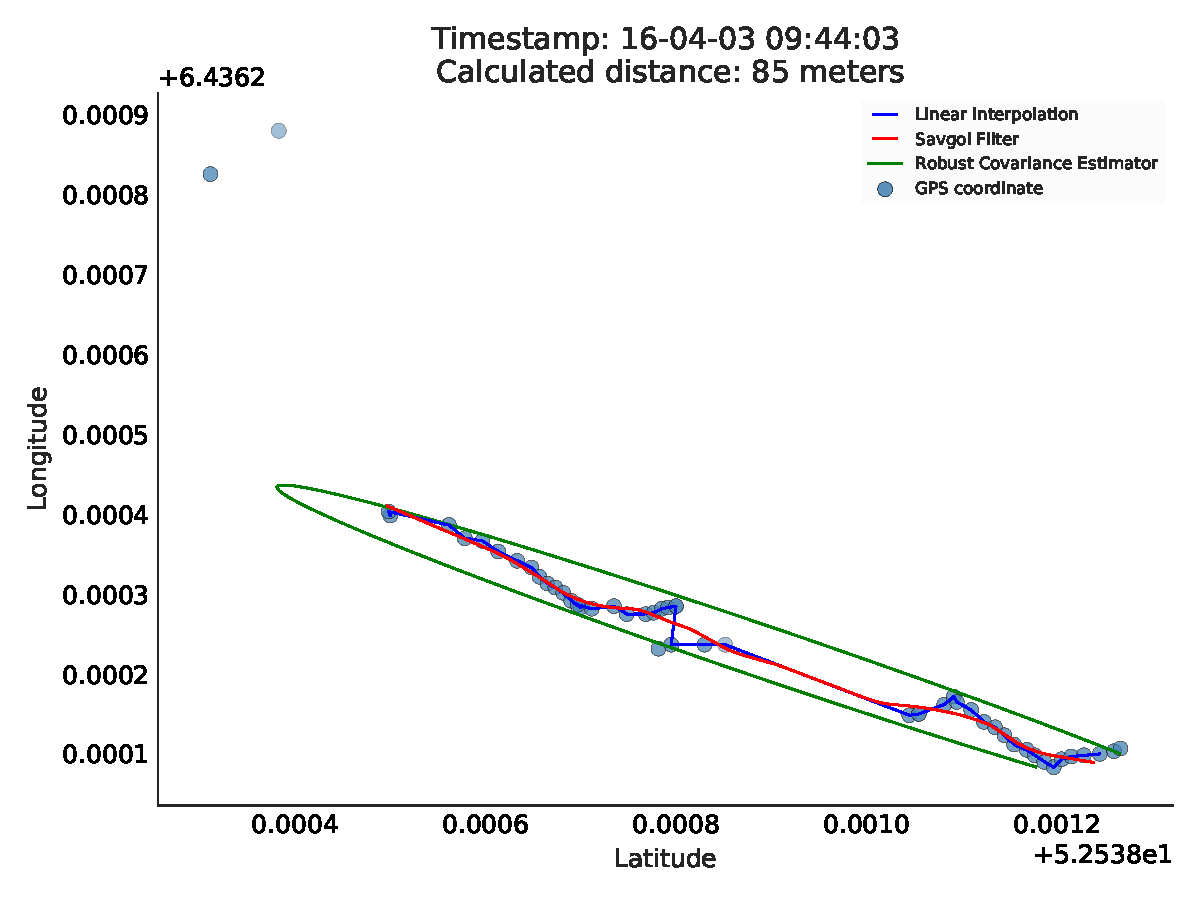
\includegraphics[scale=0.29]{gps/straight/3wAkwQDaLY7gYrhPi}
	}
	\hspace{0.5cm}
	\subfloat[]{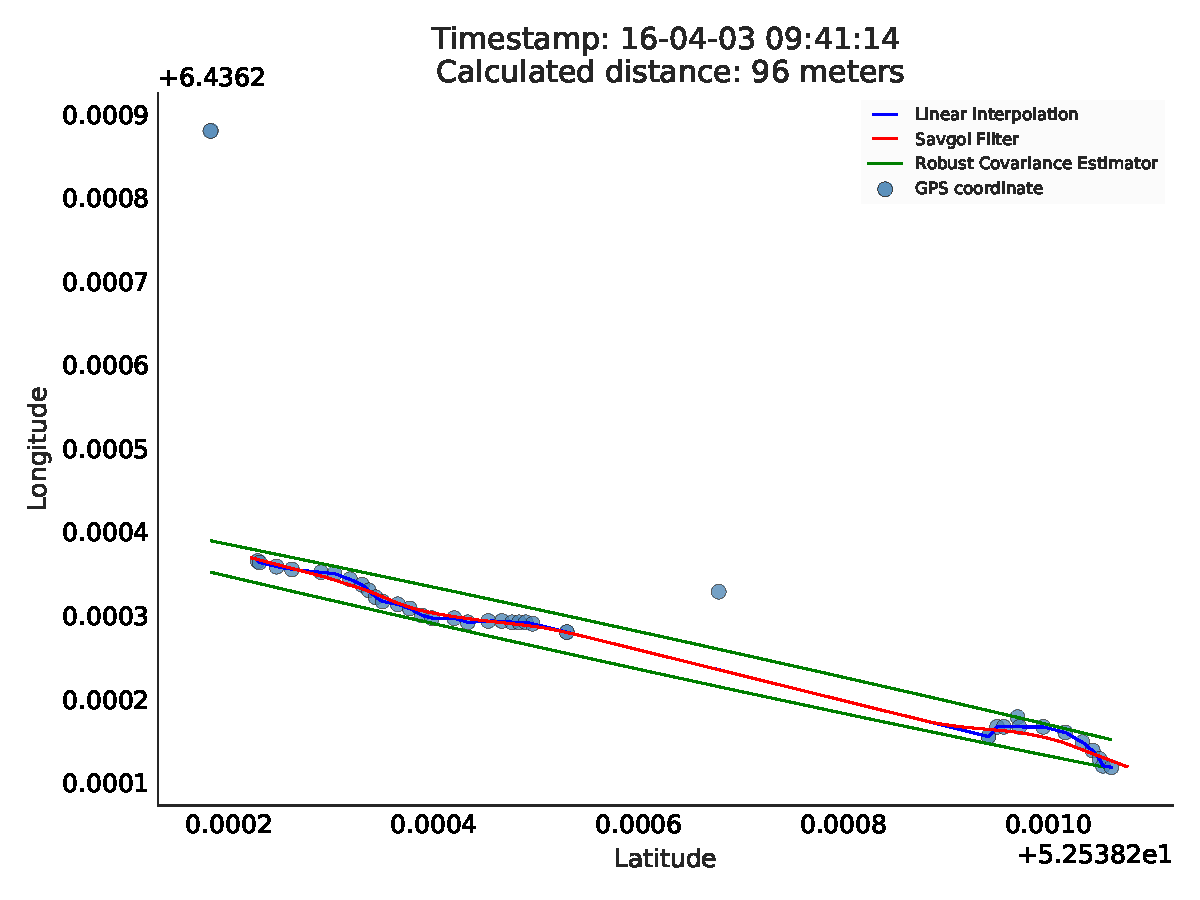
\includegraphics[scale=0.29]{gps/straight/9cuCTXcBBK2J32PoE}
	}
	\vfill
	\subfloat[]{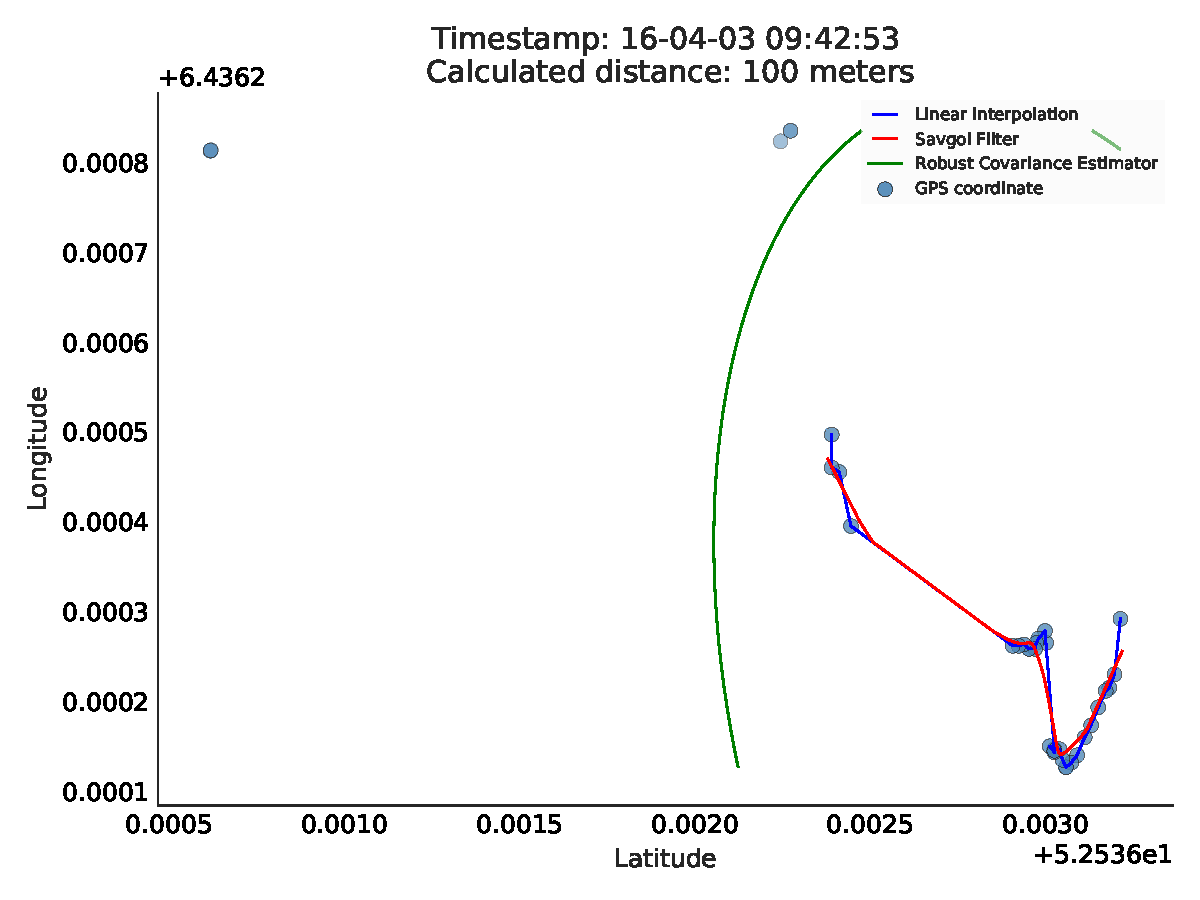
\includegraphics[scale=0.29]{gps/straight/Ba8aoCEfdhz2nxYq9}
	}
	\hspace{0.5cm}
	\subfloat[]{\label{fig:Terrible GPS Coordinates 1}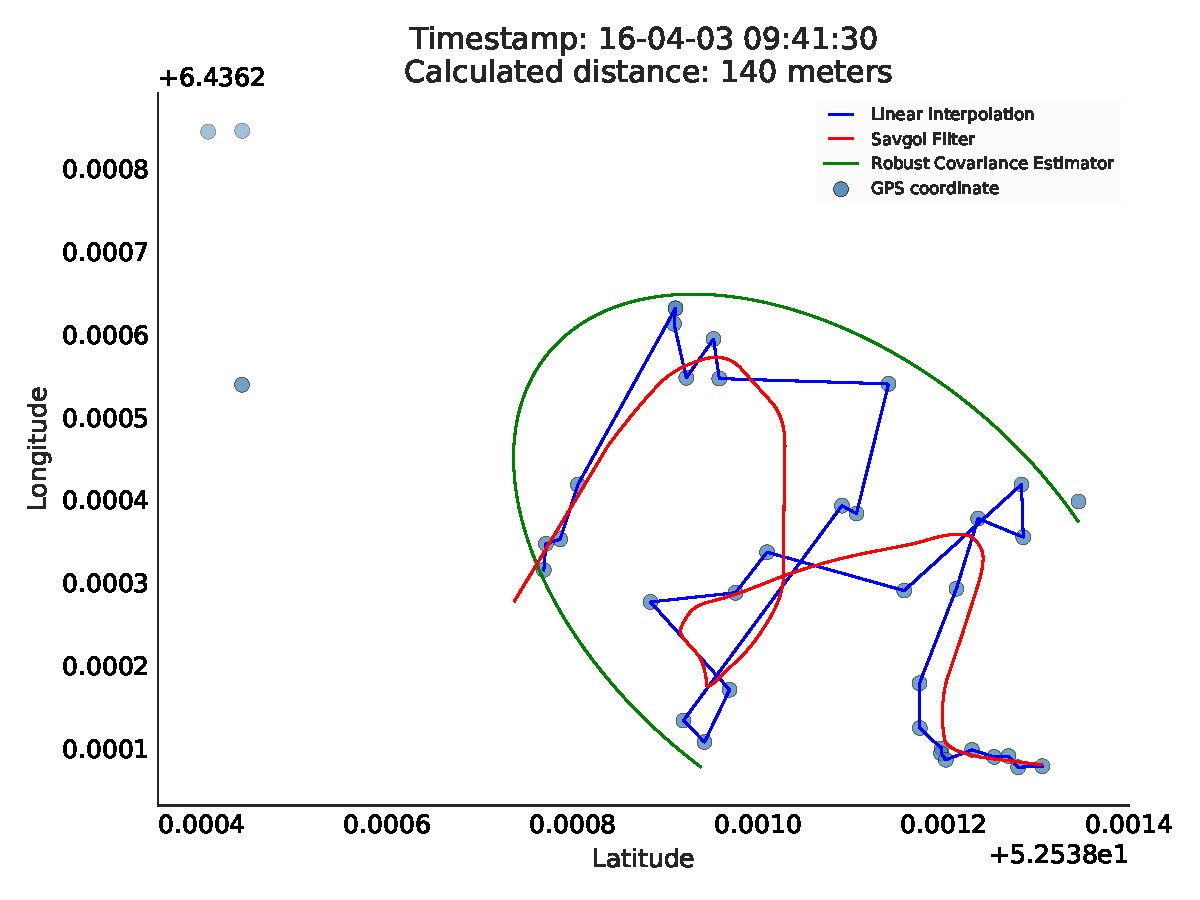
\includegraphics[scale=0.29]{gps/straight/CbpZDcgq8d6BCy5mj}
	}
	\captionof{figure}{Plots of the GPS coordinates of the walking test before and after smoothing. First, outlier detection is done using Elliptic Envelope. Afterwards, inliners are  smoothed in two stages: `Lineair Interpolation' is the first smoothing step and `Savgol Filter' the last.}
	\label{GPS Plots Straight Line}
\end{figure}
%
\begin{figure}[H]
	\ContinuedFloat 
	\centering
	\subfloat[]{\label{fig:Terrible GPS Coordinates 2}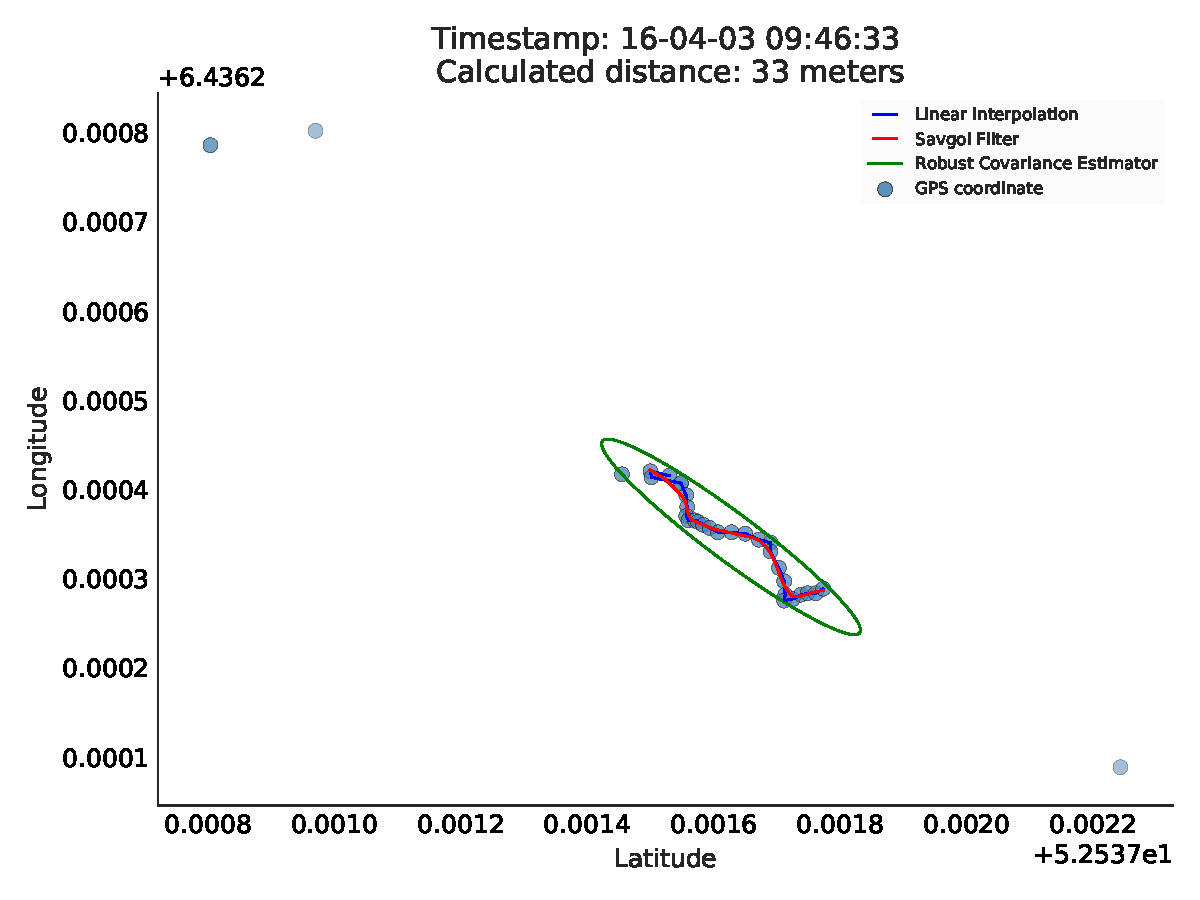
\includegraphics[scale=0.29]{gps/straight/exCkb4K2cCaZHHg4b}
	}
	\hspace{0.5cm}
	\subfloat[]{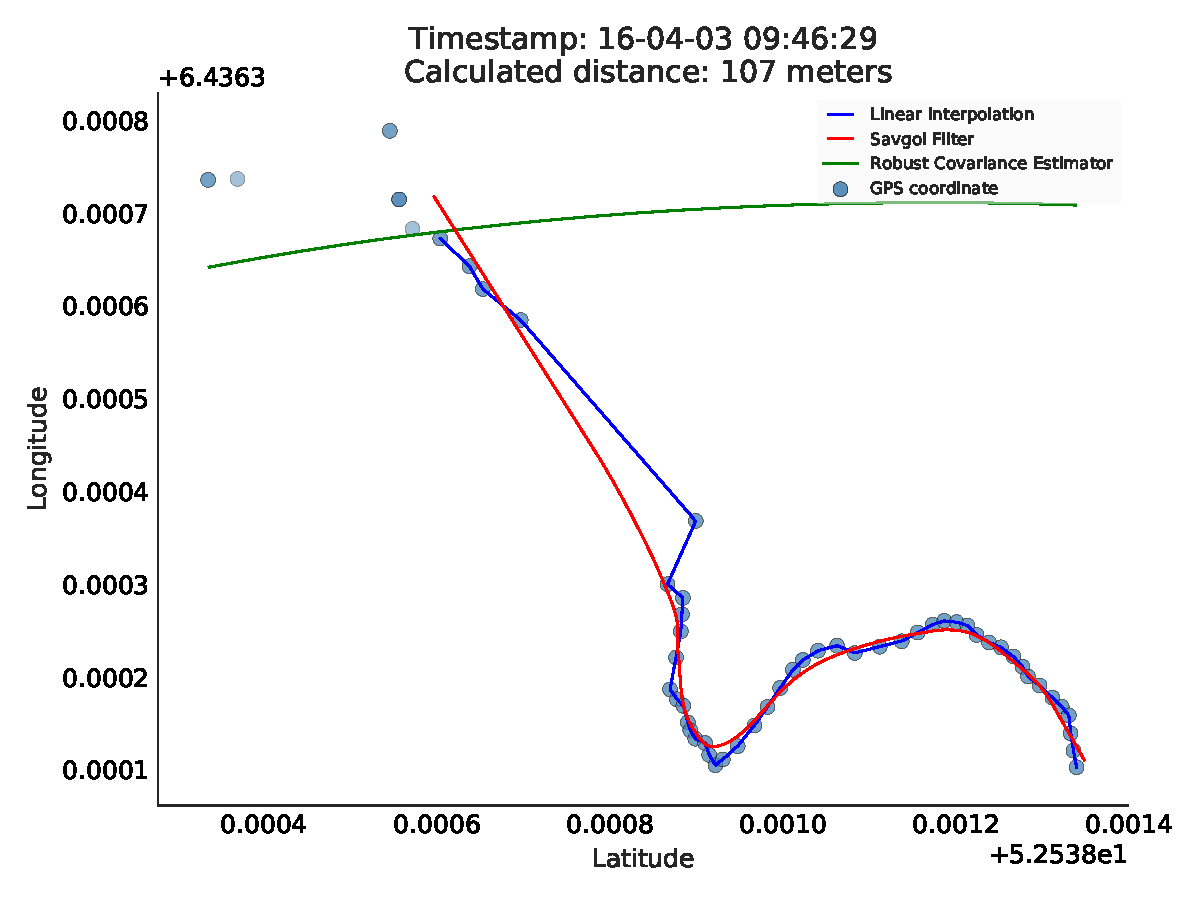
\includegraphics[scale=0.29]{gps/straight/fA2QJHC6iPcAmnu4x}
	}
	\vfill
	\subfloat[]{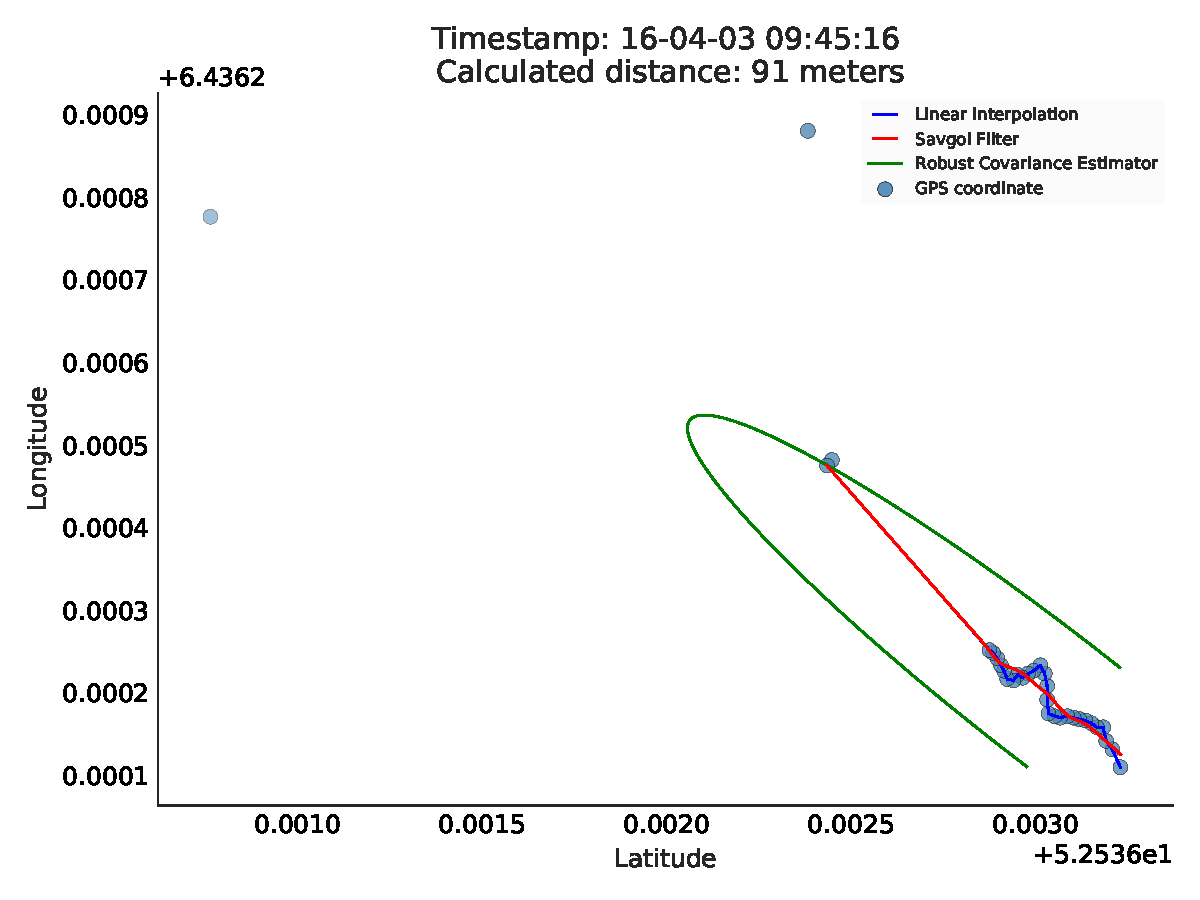
\includegraphics[scale=0.29]{gps/straight/g7zX6A4FnTu4L975N}
	}
	\hspace{0.5cm}
	\subfloat[]{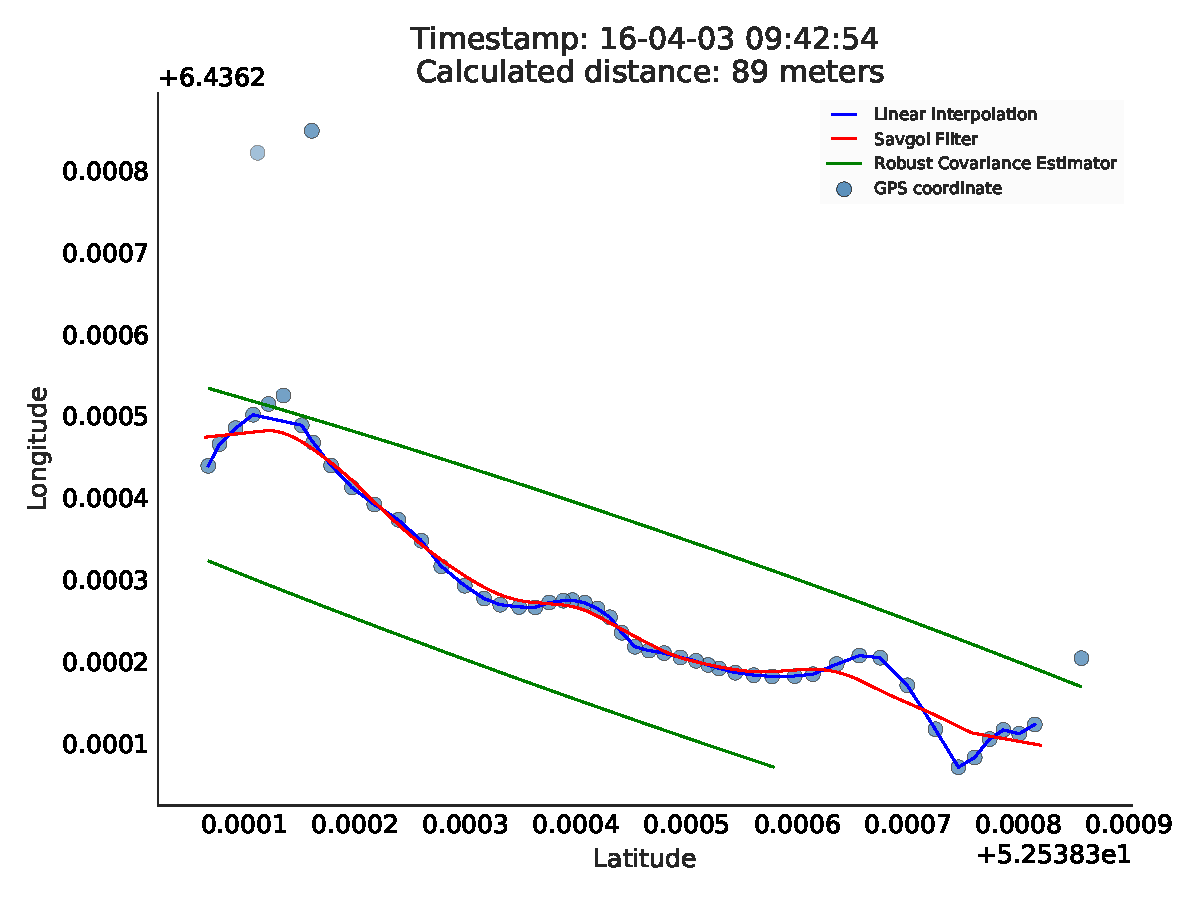
\includegraphics[scale=0.29]{gps/straight/KFb4FtR8Jjb6Ajtdc}
	}
	\vfill
	\subfloat[]{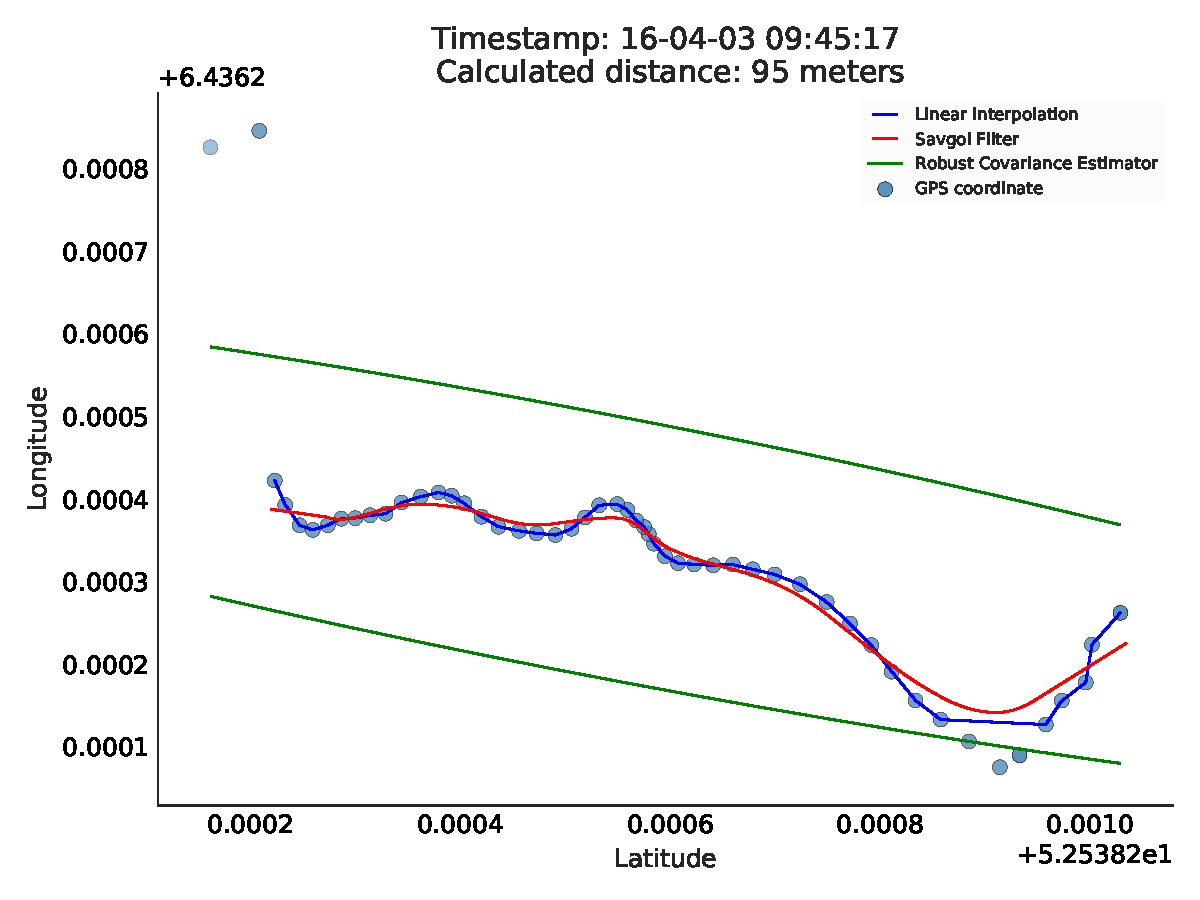
\includegraphics[scale=0.29]{gps/straight/QXtSsihbjmWnG854C}
	}
	\hspace{0.5cm}
	\subfloat[]{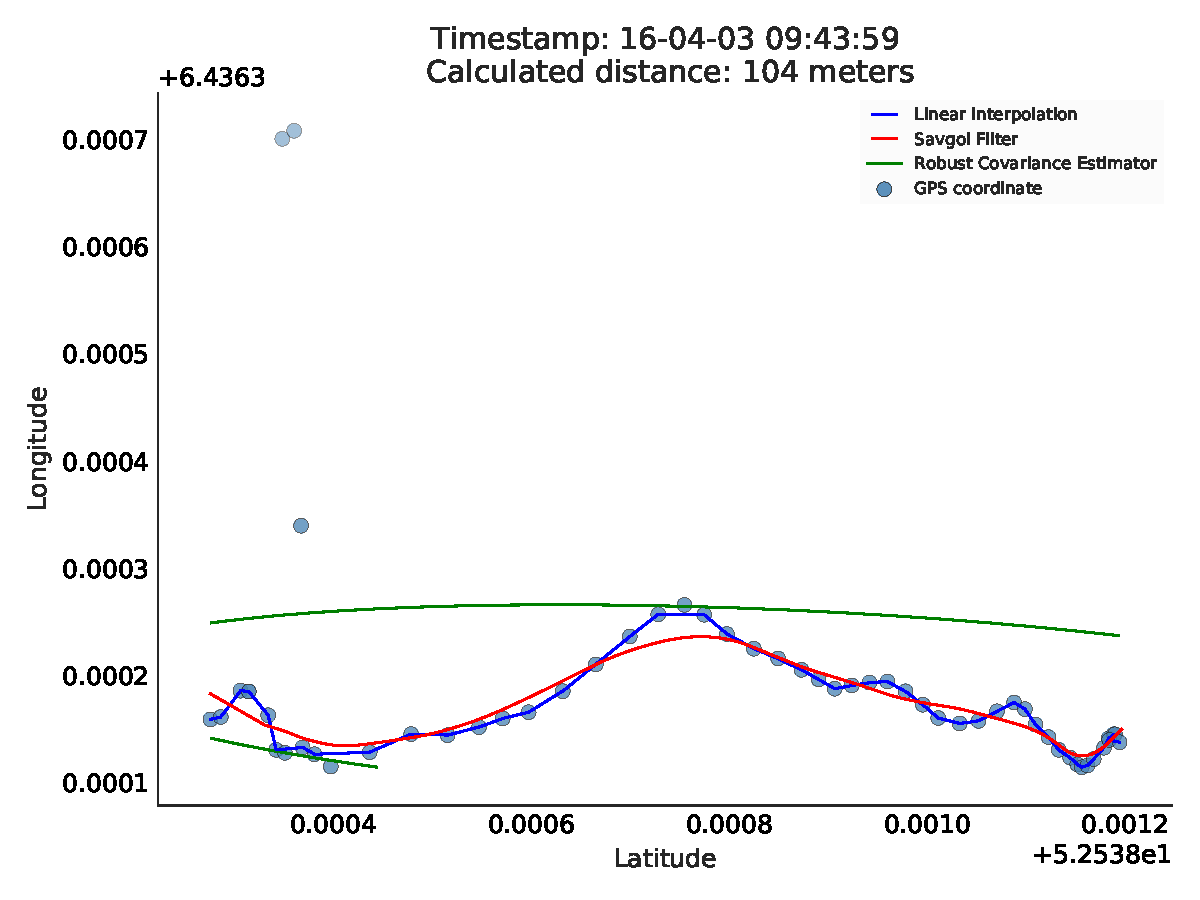
\includegraphics[scale=0.29]{gps/straight/vGn6KLTyNqBEH25YN}
	}
	\captionof{figure}{}
\end{figure}

\newpage

\section{GPS Plots Circular Path}
\begin{figure}[H]
	\centering
	\subfloat[]{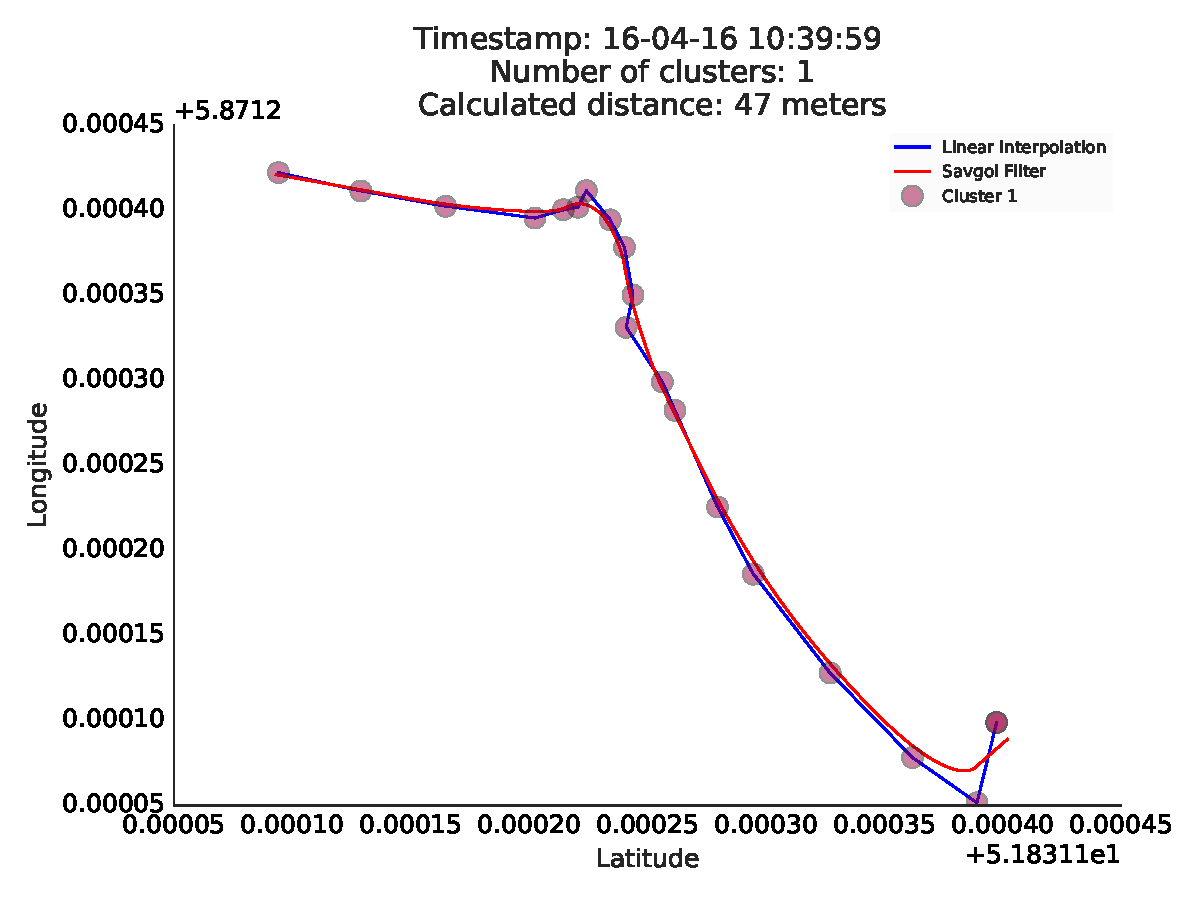
\includegraphics[scale=0.29]{gps/circle/2Zye5dTxYRNq7K7se}
	}
	\hspace{0.5cm}
	\subfloat[]{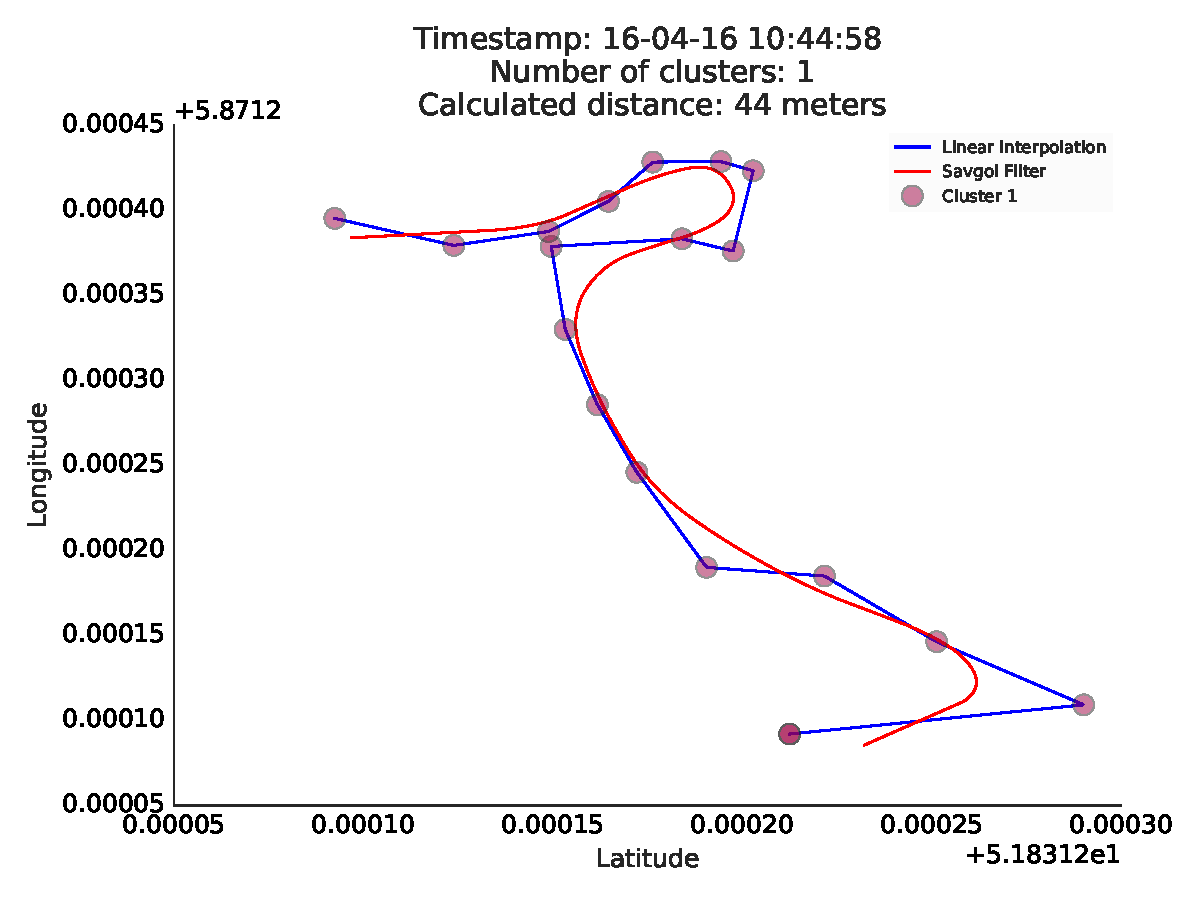
\includegraphics[scale=0.29]{gps/circle/4E2jhxMF392sEjWJF}
	}
	\vfill
	\subfloat[]{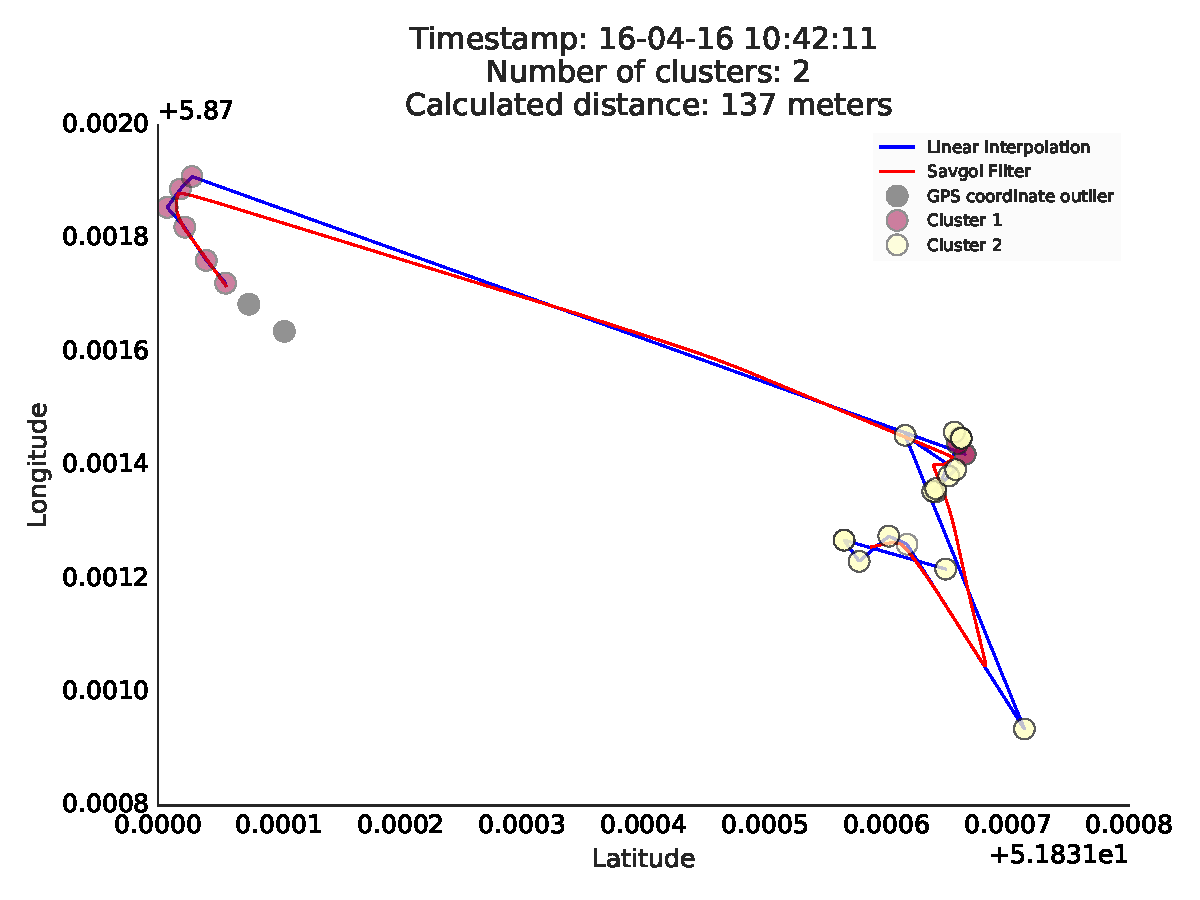
\includegraphics[scale=0.29]{gps/circle/HFgtoEcsXcmiDZHtY}
	}
	% Was eerst 141m door fout, nu 137
	\hspace{0.5cm}
	\subfloat[]{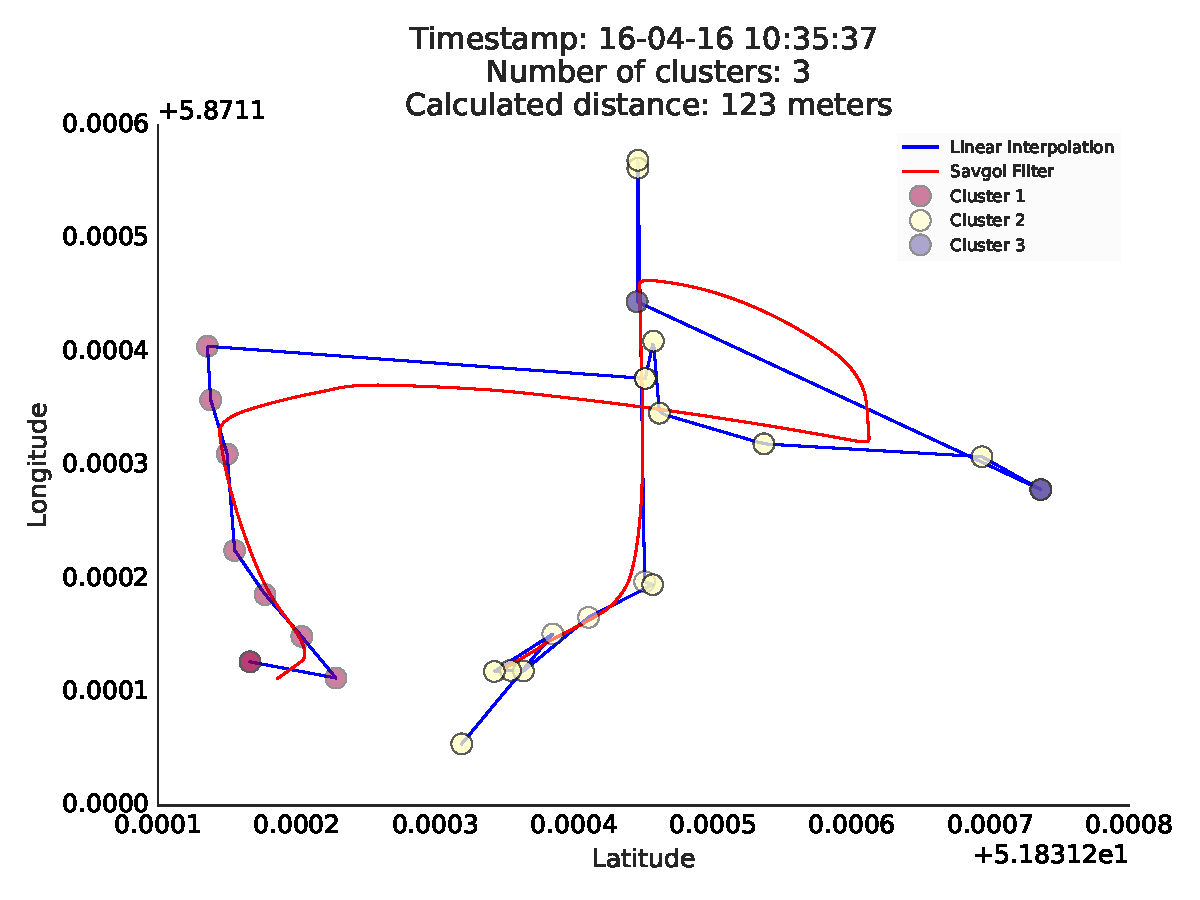
\includegraphics[scale=0.29]{gps/circle/otZE8i4oahYFNdegA}
	}
	\vfill
	\subfloat[]{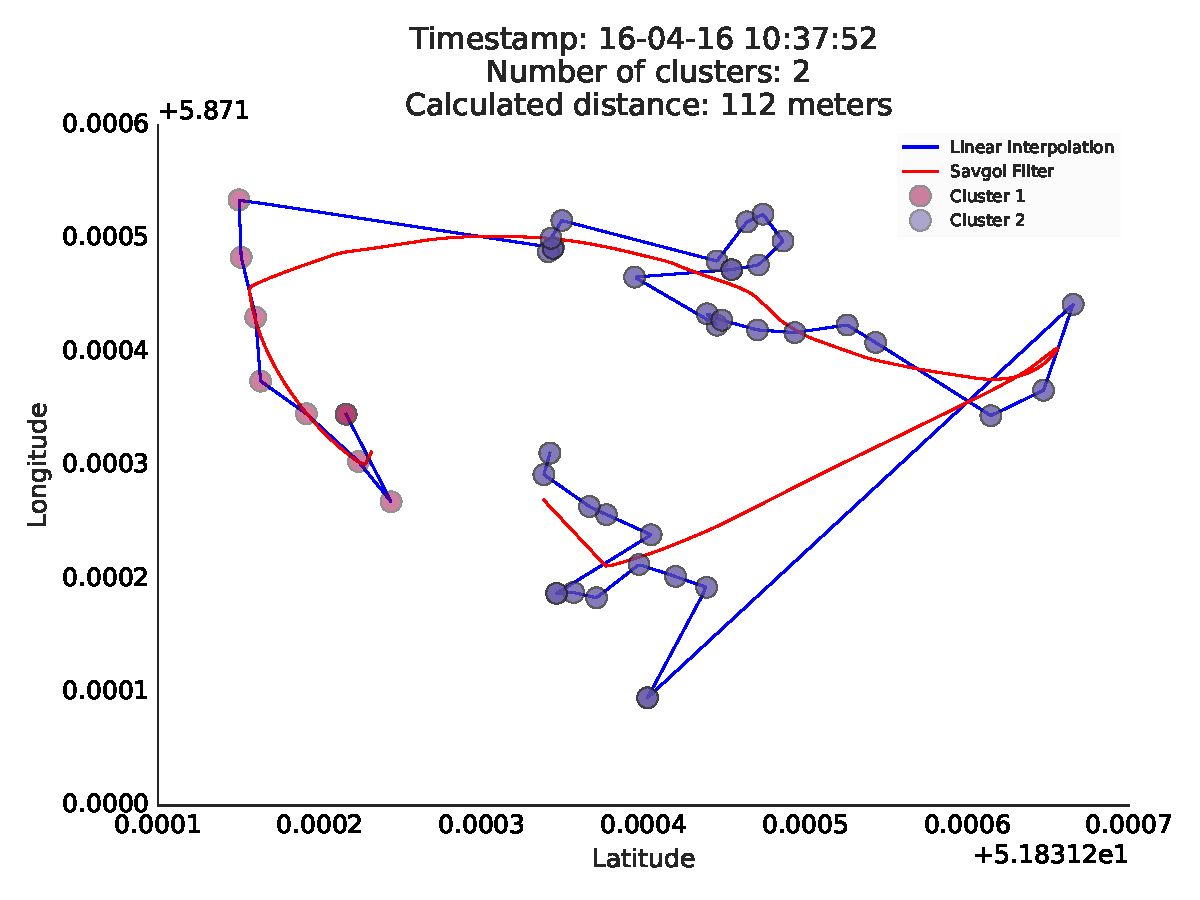
\includegraphics[scale=0.29]{gps/circle/Px5F2nQ9iaYACpJXG}
	}
	\captionof{figure}{Plots of the GPS coordinates of the walking test using a circular track. First, clustering is used to filter out the outliers. Afterwards, inliners are  smoothed in two stages: `Lineair Interpolation' is the first smoothing step and `Savgol Filter' the last. Black points are points classified as noise.}
\end{figure}

\newpage

\section{Heart Rate Boxplots}
\begin{figure}[H]
	\centering
	\subfloat[]{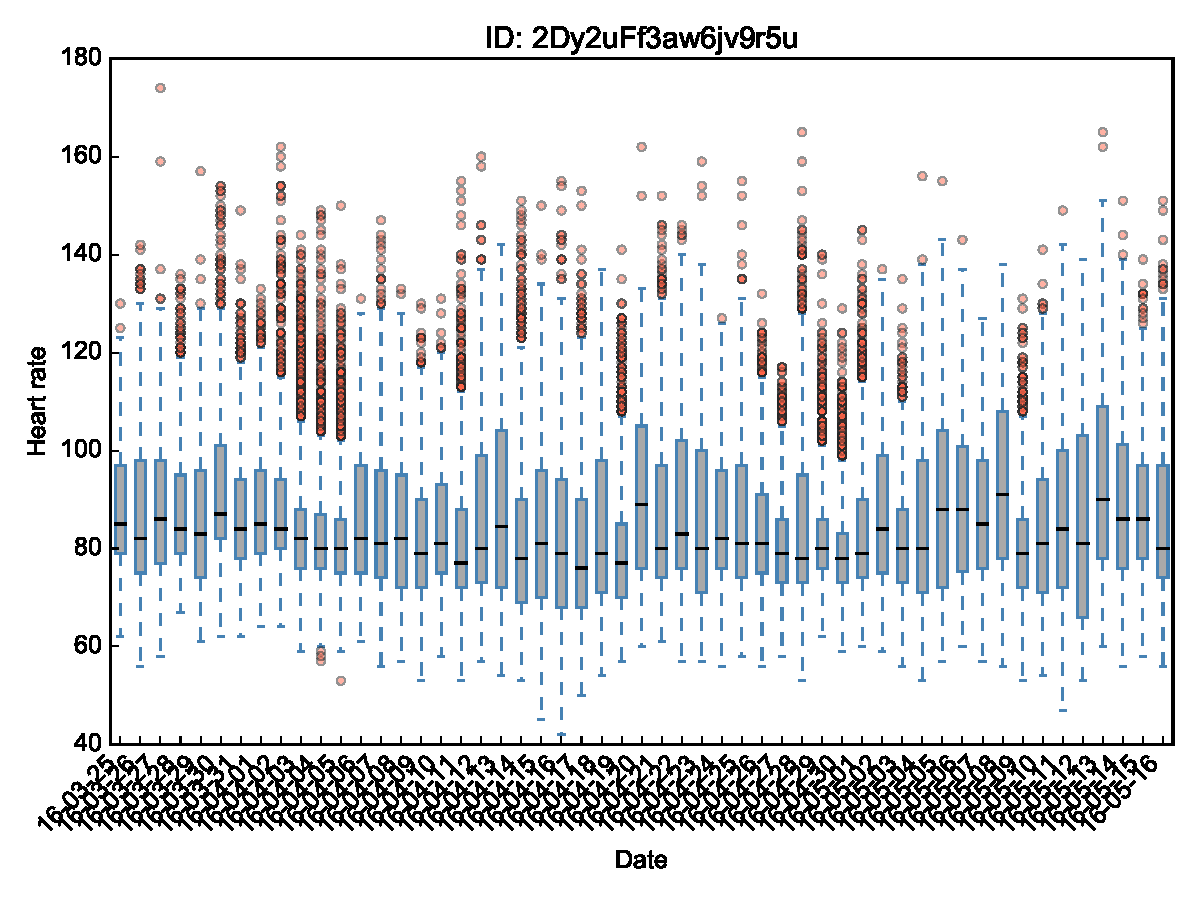
\includegraphics[scale=0.5]{boxplots/2Dy2uFf3aw6jv9r5u}
	}
	\vfill
	\subfloat[]{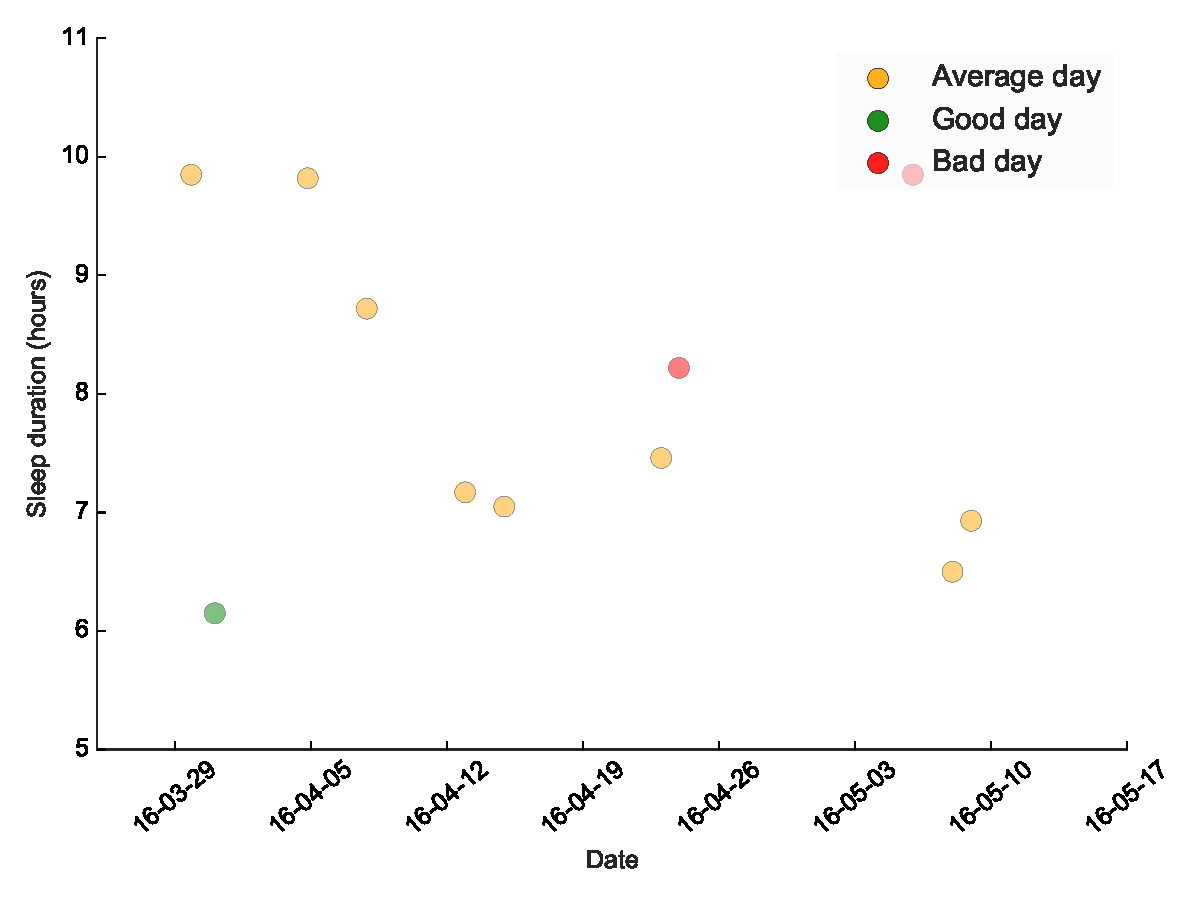
\includegraphics[scale=0.5]{boxplots/dW4YzJQEaidmyhsuY}
	}
	\captionof{figure}{Boxplots of the heart rates for each day.}
	\label{fig: heart rates boxplots}
\end{figure}

\begin{figure}
	\ContinuedFloat
	\centering
	\subfloat[]{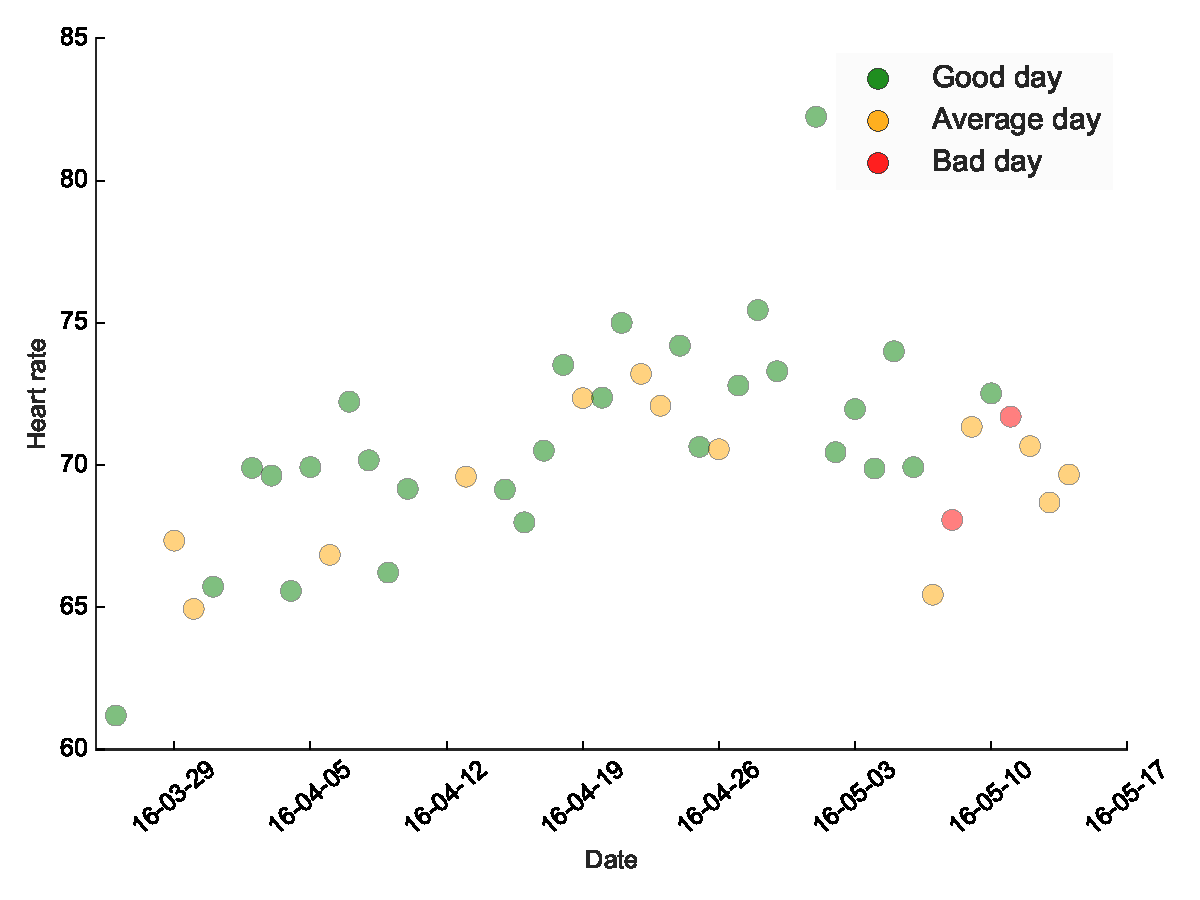
\includegraphics[scale=0.5]{boxplots/gGSWzh5PnqgFdCpq4}
	}
	\vfill
	\subfloat[]{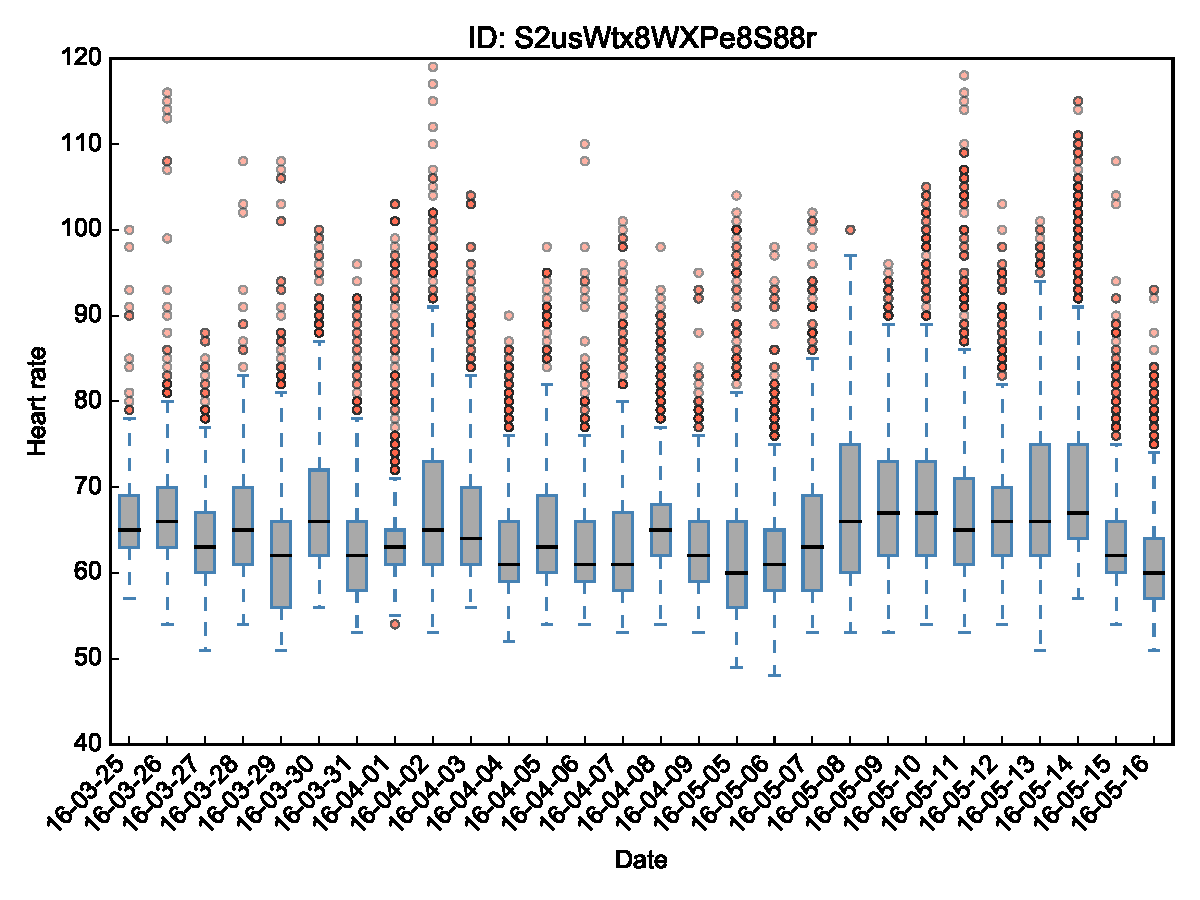
\includegraphics[scale=0.5]{boxplots/S2usWtx8WXPe8S88r}
	}
	\captionof{figure}{}
\end{figure}

\newpage

\section{Elliptic Outlier Detection}
%
\begin{code}
	\inputminted[firstline=34, lastline=95, linenos=true, fontsize=\footnotesize, breaklines=true]{python}{code/ms-analysis/WalkingTest.py}
	\caption{Code used for detecting outliers in a straight path.}
	\label{GPS Smoothing Code Straight Line}
\end{code}
%

\newpage

\section{Clustering Outlier Detection}
%
\begin{code}
	\inputminted[firstline=17, lastline=104, linenos=true, fontsize=\footnotesize, breaklines=true]{python}{code/ms-analysis/Clustering.py}
	\caption{Code used for detecting outliers in a non-straight path.}
	\label{GPS Smoothing Code Non-Straight Line}
\end{code}
%

\newpage

\section{Calculation of Walking Speed}
%
\begin{code}
	\input{code/"Walking speed".tex}
	\caption{Code used for calculating the walking speed between GPS coordinates.}
	\label{walk test code snippet}
\end{code}
%


\section{Tables}
\subsection{Sleep}
% !TeX spellcheck = en_US
% !TeX root = ../BachelorThesis.tex

\begin{table}[H]
 	\centering
 	\begingroup
 	\fontsize{6pt}{6pt}
 	\selectfont
 	\subfloat[]{
 		\csvautobooktabular[head to column names, table head=\toprule \bfseries Date & \bfseries Rating & \bfseries Duration (h)\\\midrule]
 		{csv/sleep/2Dy2uFf3aw6jv9r5u.csv}
 		\label{table:sleepduration1}
 	}
 	\hspace{1cm}
 	\subfloat[]{
 		\csvautobooktabular[head to column names, table head=\toprule \bfseries Date & \bfseries Rating & \bfseries Duration (h)\\\midrule]
 		{csv/sleep/dW4YzJQEaidmyhsuY.csv}
 		\label{table:sleepduration2}
 	}
 	\captionof{table}{Measurements of the sleep duration of our participants.} 
	\label{table: Sleep Analysis}
	
	\endgroup
\end{table}

\begin{table}[H]
	\ContinuedFloat
	\centering
 	\begingroup
 	\fontsize{6pt}{6pt}
 	\selectfont
 	\subfloat[]{
 		\csvautobooktabular[head to column names, table head=\toprule \bfseries Date & \bfseries Rating & \bfseries Duration (h)\\\midrule]
 		{csv/sleep/gGSWzh5PnqgFdCpq4.csv}
 		\label{table:sleepduration3}
 	}
 	\hspace{1cm}
 	\subfloat[]{
 		\csvautobooktabular[head to column names, table head=\toprule \bfseries Date & \bfseries Rating & \bfseries Duration (h)\\\midrule]
 		{csv/sleep/S2usWtx8WXPe8S88r.csv}
 		\label{table:sleepduration4}
 	}
 	\captionof{table}{}
	\endgroup
\end{table}
\subsection{Heart Rate}
\input{tables/"heart rate"}
\subsection{Walking Test}
\input{tables/"walking test"}


